\section[Determinanten II]{Determinanten, Matrizen und Inversion}
\Einleitung{Bereits gegen Ende des letzten Semesters habt ihr Determinanten und deren gruppentheoretischen Hintergrund kennengelernt.\\
Letzteren schauen wir uns nun verknüpft mit einer kleinen Wiederholungseinheit erneut an und erweitern unseren Werkzeugkasten mit dem Laplace'schen Entwicklungssatz, der eine weitere Möglichkeit darstellt, vor allem größere Determinanten zu berechnen. Bereits nächste Woche werden wir sehen, dass die Determinante bei der Bestimmung spezieller mit linearen Abbildungen verknüpfter Werte nützlich ist.\\
Zudem schauen wir uns an, wie man Matrizen invertieren kann und welche Feinheiten man dabei beachten muss.}

\subsection{Kurze Wiederholung zu Gruppen und deren Anwendung}
Auch wenn ihr letztes Semester bereits die wichtigsten Begriffe für Gruppen kennengelernt habt, wollen wir, bevor es richtig losgeht, hier nochmal daran erinnern. Diese neue algebraische Struktur (neben Körpern und Vektorräumen) braucht ihr im Rahmen der Mathevorlesungen vor allem zur präzisen Formulierung der Determinanten. Aber auch in der Physik spielen sie eine tragende Rolle, zum Beispiel wenn es um die Beschreibung von Symmetrien (Drehung, Verschiebung, Spiegelung etc.) geht. Daher handelt es sich hier keineswegs um ein Nischenthema sondern um ein mathematisches Werkzeug, dass zu immensen Fortschritten im Verständnis der Natur geführt hat. \\

Also dann legen wir mal los: was war denn noch gleich eine Gruppe? Dazu schauen wir uns erstmal die trockene Definition an:
\begin{Wiederholung}
{Gruppen}
Eine Gruppe besteht aus einer Menge $G$ und einer Verknüpfung $\cdot:G\times G \mapsto G$, die folgende Eigenschaften erfüllen: \\

\begin{itemize}
    \item $(u\cdot v)\cdot w = u\cdot (v\cdot w) \qquad \forall u,v,w \in G$ \qquad (Assoziativität)
    \item $\exists e\in G: u\cdot e = e\cdot u = u \qquad \forall u\in G$ \qquad (Existenz des neutralen Elements)
    \item $\forall u\in G \, \exists u^{-1} \in G\,: u\cdot u^{-1} = u^{-1} \cdot u = e$ \qquad (Existenz des inversen Elements) \\
\end{itemize} 

Ist die Verknüpfung zusätzlich noch kommutativ, spricht man von einer \red{abelschen Gruppe}.
\end{Wiederholung}
Wie sehen jetzt aber Mengen aus, die diese Voraussetzungen erfüllen und was macht sie so besonders? Dazu schauen wir und mal ein paar Beispiele an, die ihr auch schon aus dem letzten Semester kennen solltet:
\begin{Beispiel}
{Besondere Gruppen}
\begin{enumerate}
    \item Bijektive Abbildungen bilden zusammen mit der Komposition \glqq $\circ$ \grqq eine Gruppe. Dass die Komposition Assoziativität erfüllt, haben wir in Mathe 1 gesehen. Mit der Identität $\Id$ und der Umkehrabbildung sind auch neutrales und inverses Element gegeben. Wir schreiben die Gruppe als:
    \begin{equation*}
        \Bij(X)=\Menge{\varphi : X \rightarrow X}{\varphi \text{ bijektiv}}.
    \end{equation*}
    Ist $X$ eine endliche Menge, nennt man $\sigma \in \Bij(X)$ eine \red{Permutation}.
    \item Die symmetrische Gruppe \red{(wichtig!)} ist definiert als
    \begin{equation*}
        S_{n} = \Bij(\{1,...,n\}).
    \end{equation*}
    Sie enthält Abbildungen, die alle n Elemente einer Gruppe nehmen und umordnen (permutieren).
    \item Ist $X=V$ ein Vektorraum, nennt man 
    \begin{equation*}
        \Aut(V) = \Bij(V)
    \end{equation*}
    die Automorphismengruppe.
    \item Ist $V$ endlichdimensional, dann ist 
    \begin{equation*}
        \GL(V) = \Aut (V)
    \end{equation*}
    die allgemeine lineare Gruppe (\underline{G}eneral \underline{L}inear Group).
    Ist $V=\mathbb{K}^{n}$, dann gilt:
    \begin{equation*}
        \GL(n,\mathbb{K}) = \Menge{A\in \Met (n,\mathbb{K})}{\ker (A)=0}
    \end{equation*}
    \item Zusätzlich (nicht in der Vorlesung!) betrachten wir noch die spezielle lineare Gruppe, die definiert ist durch
    \begin{equation*}
        \SL(n,\mathbb{K}) = \Menge{A\in \Met (n,\mathbb{K})}{\det (A)=1}.
    \end{equation*}
    Sie enthält alle orientierungs- und volumenerhaltenden Abbildungen und ist gelegentlich ganz nützlich.
    \item (Vorgriff) Aus physikalischer Sicht spielen auch die unitäre und spezielle unitäre Gruppe mit $\mathbb{K}=\mathbb{C}$ eine wichtige Rolle
    \begin{equation*}
        \text{U}(n)=\Menge{A\in\Met (n,\mathbb{C})}{AA^{\dagger}=A^{\dagger}A=\mathds{1}_{n}} 
    \end{equation*}
    \begin{equation*}
        \text{SU}(n)=\Menge{A\in \Met (n,\mathbb{C})}{AA^{\dagger}=A^{\dagger}A=\mathds{1}_{n} \land \det (A) = 1}
    \end{equation*}
    Tatsächlich bilden diese beiden Gruppen die Grundlage des Standardmodells der Teilchenphysik! Solltet ihr mit dem Symbol $\dagger$ (sprich \glqq{}dagger\grqq{}) noch nichts anfangen können, seid beruhigt: ihr lernt es gleich zu beginn dieser Vorlesung kennen. Es bedeutet, dass man die Matrix komplex konjugiert und transponiert.
\end{enumerate} 
\end{Beispiel}
Anhand dieser Beispiele seht ihr schon, dass die Gruppenstruktur in unter Anderem durch bijektive Abbildungen gegeben ist. Bijektivität ist deswegen wichtig, da wir ein inverses Element, sprich eine Umkehrabbildung brauchen. Geben wir ein paar weitere Schranken vor, enthalten wir speziellere Gruppen wie die symmetrische Gruppe oder die Automorphismengruppe. \\
Permutationen, die Elemente einer endlichen Menge umordnen, oder auch Symmetrietransformationen, sind am Ende nichts anderes als bijektive Abbildungen. Eine Umordnung kann man immer zurückordnen und eine Transformation, wie zum Beispiel eine Drehung oder eine Verschiebung, lässt sich immer zurücktransformieren. Hoffentlich macht das die Bedeutung von Gruppen etwas klarer. \\

Als nächstes wollen wir nochmal ein paar wichtige Begriffe, die im Zusammenhang mit Gruppen stehen, wiederholen.
\begin{Wiederholung}
{Gruppenhomomorphismus}
Ein Gruppenhomomorphismus $\varphi: G \rightarrow H$ zwischen zwei Gruppen $G$ und $H$ erfüllt die Bedingung
\begin{equation*}
    \varphi (a\cdot b)=\varphi (a) \cdot \varphi (b) \quad a,b \in G 
\end{equation*}
\end{Wiederholung}
\begin{Wiederholung}
{Transposition}
Eine \red{Transposition} ist eine bestimmte Permutation, die wie folgt definiert ist:
\begin{equation*}
    \tau_{ij} := \Matrix{1 & ... & i & ... & j & ... & n \\ 1 & ... & j & ... & i & ... & n}.
\end{equation*}
Sie vertauscht also die Elemente $i$ und $j$ einer gegebenen (nummerierten) Anzahl von Elementen miteinander.
\end{Wiederholung}
\begin{Wiederholung}
{Signum}
Das \red{Signum} einer Permutation $\sigma$ ist ein Gruppenhomomorphismus $\epsilon : S_{n} \rightarrow \{-1,1\}$, der definiert ist durch
\begin{equation*}
    \epsilon (\sigma) := \prod_{i<j} \frac{\sigma(j)-\sigma(i)}{j-i}
\end{equation*}
Jede Permutation lässt sich durch eine Verkettung von Transpositionen darstellen:
\begin{equation*}
    \sigma = \tau_{1}\circ\tau_{2} \circ ... \circ \tau_{k}.
\end{equation*}
Dabei ist die Anzahl $k$ der Transpositionen nicht eindeutig. Was aber sehr wohl eindeutig ist, ist ob $k$ gerade oder ungerade ist. Man kann tatsächlich zeigen, dass das Signum auch berechnet werden kann durch
\begin{equation*}
    \epsilon(\sigma)=(-1)^{k},
\end{equation*}
was deutlich leichter ist als die Formel, die wir davor hatten.
\end{Wiederholung}
\begin{Wiederholung}
{Zykel}
Ein \red{Zykel} ist eine weitere spezielle Permutation, die wie folgt definiert ist:
\begin{equation*}
    \zeta = \Matrix{1 & 2 & ... & n} = [2\,3\, ... \, n] = \Matrix{1 & 2 & ... & n-1 & n \\ 2 & 3 & ... & n & 1}.
\end{equation*}
Er bewirkt also eine zyklische Vertauschung aller Elemente. Möglicherweise ist euch der Begriff schonmal über den Weg gelaufen, falls ihr das Levi-Civita-Symbol (Epsilon-Tensor) im ersten Semester behandelt habt.
\end{Wiederholung}
Falls ihr zu diesen Begriffene weitere Beispiele sehen wollt, könnt ihr gerne in die Notizen zum Mathe 1 - Tutorium schauen. Hier wollen wir uns jetzt ein paar Anwendungen der Gruppentheorie anschauen. An erstere Stelle steht dabei natürlich die Definition der Determinante.
\begin{Beispiel}
{Anwendung von Gruppen (1/2) - Die Determinante}
Wie ihr (hoffentlich) bereits in Mathe 1 gelernt habt, ist die Determinante eine Abbildung $\det : \Met(n,\mathbb{K} \rightarrow \mathbb{K})$, die folgende Axiome erfüllt:
\begin{enumerate}
    \item Die Determinante ist linear in jeder Spalte ($\lambda, \mu \in \mathbb{K}):$
    \begin{align*}
        \det&\Matrix{a_{1} & ... & a_{i-1} & \lambda a_{i}+\mu b_{i} & a_{i+1} & ... & a_{n}} \\ &= \lambda \det \Matrix{a_{1} & ... & a_{i} & ... & a_{n}} + \mu \det \Matrix{a_{1} & ... & b_{i} & ... & a_{n}},
    \end{align*}
    wobei $a_{i}$ und $b_{i}$ n-dimensionale Spaltenvektoren sind.
    \item Die Determinante ist alternierend, d.h. $\det A = 0$, falls zwei Spalten von $A$ gleich sind:
    \begin{equation*}
        \rg (A) < n \quad \Rightarrow \quad \det (A) = 0. 
    \end{equation*}
    (Erinnerung: Rang = Dimension des Bildes).
    \item Die Determinante bildet die Identität auf $1$ ab:
    \begin{equation*}
        \det (\mathds{1}_{n}) = 1
    \end{equation*}
\end{enumerate}
Spannenderweise existiert eine Funktion, die diese Axiome erfüllt und zudem eindeutig ist. Sie ist durch die monströse Leibnizsche Determinantenformel gegeben. Sei dazu $A\in \Met (n, \mathbb{K})$:
\begin{equation*}
    \det (A) = \sum_{\sigma \in S_{n}} \epsilon (\sigma) a_{\sigma(1)1}\cdot ... \cdot a_{\sigma(n)n}.
\end{equation*}
Anhand dieser Formel wird klar, warum wir Gruppen für die Berechnung von Determinanten brauchen. Wir müssen hier nämlich über sämtliche Permutationen der symmetrischen Gruppe $S_{n}$ summieren! Leider sind das genau $n!$ Stück, womit man für größere Matrizen eine enorme Anzahl an Summanden bekommt (bei 6x6-Matrizen sind es zum Beispiel stolze 720!). Zum Glück habt ihr ja schon leichtere Methoden kennengelernt, mit denen man die Determinante schneller ausrechnen kann.
\end{Beispiel}
\subsubsection{Exkurs: Symmetrietransformationen}
\begin{Beispiel}
{Anwendung von Gruppen (2/2) - Symmetrietransformationen}
Das Folgende ist nicht Teil der Mathevorlesung und vor allem für Interessierte gedacht. Ein paar Sachen werden euch dabei vielleicht in den Vorlesungen zur Quantenmechanik wiederbegegnen... \\
\begin{enumerate}
\item \textbf{Translationsgruppe} \\
Schauen wir uns zunächst einmal die Translationsgruppe $T$ für eine Funktion \linebreak $f:\mathbb{R} \rightarrow \mathbb{R}$ an. Diese Gruppe besteht aus Elementen $t_{a}$, $a \in \mathbb{R}$, die wie folgt auf die Funktion wirken:
\begin{equation*}
    t_{a}f(x)=f(x+a).    
\end{equation*}
Sie verschieben also das Argument der Funktion um $a$. Es ist schnell zu erkennen, dass es ein inverses Element $t_{-a}$ und ein neutrales Element $t_{0}$ gibt, wenn wir die (assoziative) Verknüpfung wie folgt wählen:
\begin{equation*}
    t_{a}\cdot t_{b} = t_{a+b}.
\end{equation*}
Können wir nun eine spezielle Darstellung der Gruppenelemente finden? Aber klar! Dazu schauen wir uns eine infinitesimale Verschiebung $t_{da}$ an und erinnern an die Definition des Differenzenquotienten (denn wir hier mal auf Physikerart hinschreiben):
\begin{align*}
    \frac{df}{dx}=&\frac{f(x+da)-f(x)}{da} \\
    &\Rightarrow t_{da}f(x) = f(x+da) = f(x)+da \cdot \frac{df}{dx} = \big( 1 + da\frac{d}{dx} \big) f(x)
\end{align*}
Jetzt nutzen wir die Definition der Verknüpfung aus und erhalten für beliebige Transformationen:
\begin{align*}
    t_{a} = t_{\frac{a}{2}}\cdot t_{\frac{a}{2}} = ... &= \lim_{N \rightarrow \infty} \big( t_{\frac{a}{N}} \big)^{N} = \lim_{N \rightarrow \infty} \big( 1 + \frac{a}{N} \frac{d}{dx} \big)^{N} \\ 
    &= \exp{(a\frac{d}{dx})}
\end{align*}
Dabei haben wir benutzt, dass $a/N$ für große $N$ sehr klein und damit zu $da$ wird. Außerdem haben wir die Grenzwertdarstellung der Exponentialfunktion verwendet, die noch aus dem ersten Semester bekannt sein sollte. \\
Das interessante Ergebnis unserer kleinen Rechnung ist also:
\begin{equation*}
    t_{a}f(x)=\exp{(a\frac{d}{dx})}f(x) = f(x+a)
\end{equation*}
womit wir eine explizite Darstellung gefunden haben. Genau genommen nennt man das Argument der Exponentialfunktion ohne den Parameter $a$, also $d/dx$, die (Operator-)Darstellung der Translationsgruppe.

\item \textbf{Rotationsgruppe} \\
Diese Art von Rechnung ist zum Beispiel in der Quantenmechanik sehr nützlich und kann auch auf Rotationen angewendet werden. Die Rotationsgruppe ist gegeben durch die spezielle orthogonale Gruppe $\text{SO}(N)$, wobei 
\begin{equation*}
    \text{SO}(N) := \Menge{R \in \Met(n,\mathbb{R})}{RR^{T}=R^{T}R=\mathds{1} \land \det(R) = 1}.
\end{equation*}
(Wenn ihr Normen einführt werdet ihr Lernen, dass diese Matrizen die Länge eines Vektors unverändert lassen und wegen $\det(R)=1$ keine Spiegelungen enthalten). \\
Der Einfachheit halber wollen wir hier nur Rotationen um die z-Achse in drei Dimensionen betrachten, die durch die wohlbekannte Matrix
\begin{equation*}
    R_{\theta} = \Matrix{\cos(\theta) & -\sin(\theta) & 0 \\ \sin(\theta) & \cos(\theta) & 0 \\ 0 & 0 & 1}
\end{equation*}
gegeben sind. Eine Rotation $r_{\theta}$ einer Funktion $f:\mathbb{R}^{3} \rightarrow \mathbb{R}$ ist dann gegeben durch:
\begin{equation*}
    r_{\theta}f(v) = f(R_{\theta} v).
\end{equation*}
Diese Transformationen $r_{\theta}$ bilden aus denselben Gründen wie bei den Translationen eine Gruppe. \\
Können wir auch hier wieder eine explizite Darstellung finden? Aber natürlich! Dazu schauen wir uns abermals ein infinitesimale Transformation an und beachten dafür die Kleinwinkelnäherung $\sin(d\theta)=d\theta$ und $\cos(d\theta)=1$:
\begin{equation*}
    R_{d\theta}=\Matrix{1 & -d\theta & 0 \\ d\theta & 1 & 0 \\ 0 & 0 & 1}.
\end{equation*}
Daraus folgt:
\begin{equation*}
    r_{d\theta}f(v) = f(R_{d\theta}v) = f(x-yd\theta, y+xd\theta, z)
\end{equation*}
Jetzt packen wir den Zauberstab aus und spielen ein wenig mit den Differentialen herum, aber versprochen, es funktioniert! Im Differenzenquotienten packen wir erstmal einfach ein konstantes $y$ und $x$ hinzu, was uns ja keiner verbietet ($yd\theta$ ist ja immernoch sehr klein):
\begin{align*}
    \frac{df}{dx}&=\frac{f(x+(-yd\theta),y,z)-f(x,y,z)}{-yd\theta} \Leftrightarrow f(x-yd\theta,y,z)=(1-yd\theta\frac{d}{dx})f(x,y,z) \\
    \frac{df}{dy}&=\frac{f(x,y+xd\theta,z)-f(x,y,z)}{xd\theta} \Leftrightarrow f(x,y+xd\theta,z) = (1+xd\theta\frac{d}{dx})f(x,y,z)
\end{align*}
Daraus folgt, wenn wir annehmen, dass $d\theta^{2}$ sehr klein und somit vernachlässigbar ist:
\begin{align*}
    f(x-yd\theta,&y+xd\theta,z) = (1-yd\theta\frac{d}{dx})f(x,y+xd\theta,z)\\ &= (1-yd\theta\frac{d}{dx})(1+xd\theta\frac{d}{dx})f(x,y,z) = (1+xd\theta\frac{d}{dx}-yd\theta\frac{d}{dx})f(x,y,z).
\end{align*}
Wir haben also für die infinitesimale Rotation gefunden:
\begin{equation*}
    r_{d\theta}f(v)=(1+d\theta(x\frac{d}{dx}-y\frac{d}{dx}))f(v).
\end{equation*}
Das sieht doch schonmal richtig gut aus! Tatsächlich können wir hier den gleichen Trick wie bei der Translationsgruppe benutzen, um diese Vorschrift zu verallgemeinern:
\begin{align*}
    r_{\theta}f(v) = (r_{\frac{\theta}{2}})^{2}f(v)&=...=\lim_{N\rightarrow\infty}(r_{\frac{\theta}{N}})^{N}f(v)=\lim_{N\rightarrow\infty}(1+\frac{\theta}{N}(x\frac{d}{dx}-y\frac{d}{dy}))^{N}f(v)\\ &=\exp{(\theta(x\frac{d}{dy}-y\frac{d}{dx})}f(v) =: \exp{(\theta L)}f(v)
\end{align*}
Wir haben also tatsächlich eine (Operator-)Darstellung der Rotationsgruppe gefunden! Sie lautet:
\begin{equation*}
    L:=x\frac{d}{dy}-y\frac{d}{dx}.
\end{equation*}
Wir hoffen, dass diese doch etwas verschwurbelte Rechnung einigermaßen verständlich war. Sollte sie zu Verwirrung geführt haben, vergesst einfach die letzten zwei Seiten und konzentriert euch auf den wesentlichen Stoff! Vielleicht hat es ja trotzdem bei dem/der ein oder anderen, der/die auch schon Quantenmechanik (Physik 3) gehört und $L$ als den berühmten Drehimpulsoperator (oder besser gesagt seine z-Komponente) erkannt hat, zu einem Aha-Erlebnis geführt. Es sind unserer Meinung nach einfach zwei sehr schöne Beispiele für die Verwendung von Gruppen.

\end{enumerate}
\end{Beispiel}

\subsection{Kurze Wiederholung zur linearen Algebra}
Bevor wir \textit{wirklich }loslegen, wollen wir noch einmal an die wichtigsten Begriffe und Sätze rund um Vektorräume und lineare Abbildungen erinnern:
\begin{Wiederholung}
{Vektorraum und Linearkombination}
Ein \red{Vektorraum über $\mathbb{K}$}\footnote{$\mathbb{K}$ ist einfach der Körper (wie z.B. $\mathbb{R}$), aus dem die Skalare für die Multiplikation kommen.} ist eine \underline{Menge} $V$ zusammen mit der \red{vektoriellen Addition} und der \red{skalaren Multiplikation} bzgl. von $\mathbb{K}$.\\
\begin{tabular}{l|l|l}
    \textbf{Name} &\textbf{ Definition }&\textbf{ Erklärung} \\
    \hline
    Addition: & $V\times V\to V:\, (v,w)\mapsto v+w$ &\parbox[t]{5cm}{\blue{Die Summe zweier Vektoren ist wieder ein Vektor.}} \\
    Skalare Multiplikation: & $\mathbb{K}\times V\to V:\,(\lambda, v)\mapsto \lambda \cdot v$ & \parbox[t]{5cm}{\blue{Wir können Vektoren skalieren und erhalten dadurch wieder Vektoren.}}
\end{tabular}
Die Kombination aus Addition und Multiplikation verschiedener Vektoren nennen wir \red{Linearkombination}. Dies schreiben wir als
\begin{equation*}
    \boxed{v=\sum_{i=1}^r\lambda_i v_i}
\end{equation*}
\end{Wiederholung}
\begin{Wiederholung}
{Basis und Dimension}
Ein linear unabhängiges Erzeugendensystem\footnote{Mit Linearkombinationen der Vektoren der Familie müssen wir den jeden Vektor des Vektorraums erzeugen können.} eines Vektorraums nennen wir eine \red{Basis} von $V$.\\
Zusammen mit dem Satz über Eindeutigkeit hat jeder Vektor $v\in V$ eine eindeutige Darstellung bezüglich einer Basis, aber die gewählte Basis ist nicht eindeutig.\\
Hat $V$ eine endliche Basis mit $n$ Elementen, so nennen wir diese Zahl die \red{Dimension} $\dim V=n$ von $V$.\\
Ist $V=\{\Vec{0}\}$, so ist $\dim V=0$. Andererseits ist $\dim V=\infty$.
\end{Wiederholung}
\begin{Wiederholung}
{Lineare Abbildungen}
Wir nennen eine \red{Abbildung} $F$ zwischen zwei Vektorräumen\footnote{beide über dem gleichen Körper $\mathbb{K}$} $V$ und $W$, also $F:V\to W$ \red{$\mathbb{K}$-linear}, wenn sie die folgenden Eigenschaften für alle $v,w\in V$ und $\lambda\in\mathbb{K}$ erfüllt:
\begin{align*}
    F(v+w)&=F(v)+F(w)\\
    F(\lambda v)&=\lambda F(v).
\end{align*}
\end{Wiederholung}
\begin{Wiederholung}
{Kern und Bild von $F$}
Die Menge aller Vektoren aus $V$, die durch eine lineare Abbildung $F\in L(V,W)$ auf den \underline{Nullvektor} von $W$ abgebildet werden, nennen wir den \red{Kern von $F$}, geschrieben als\\
$\ker F= F^{-1}(\Vec{0})=\{v\in V\furdas F(v)=\Vec{0}\}\subseteq V$.\\
Die Menge aller Vektoren aus $W$, die wir durch $F$ abbilden können, nennen wir das \red{Bild von F}, geschrieben als\\
$\im F=F(V)\subseteq W$.
\end{Wiederholung}
Lineare Abbildungen eines Vektorraumes $V$ in sich selbst nennen wir \red{Endomorphismen}, bijektive Abbildungen $F:V\to W$ \red{Isomorphismen}. In der folgenden Zeichnung sind noch einmal die wichtigsten Begriffe zusammengefasst.
\begin{center}
    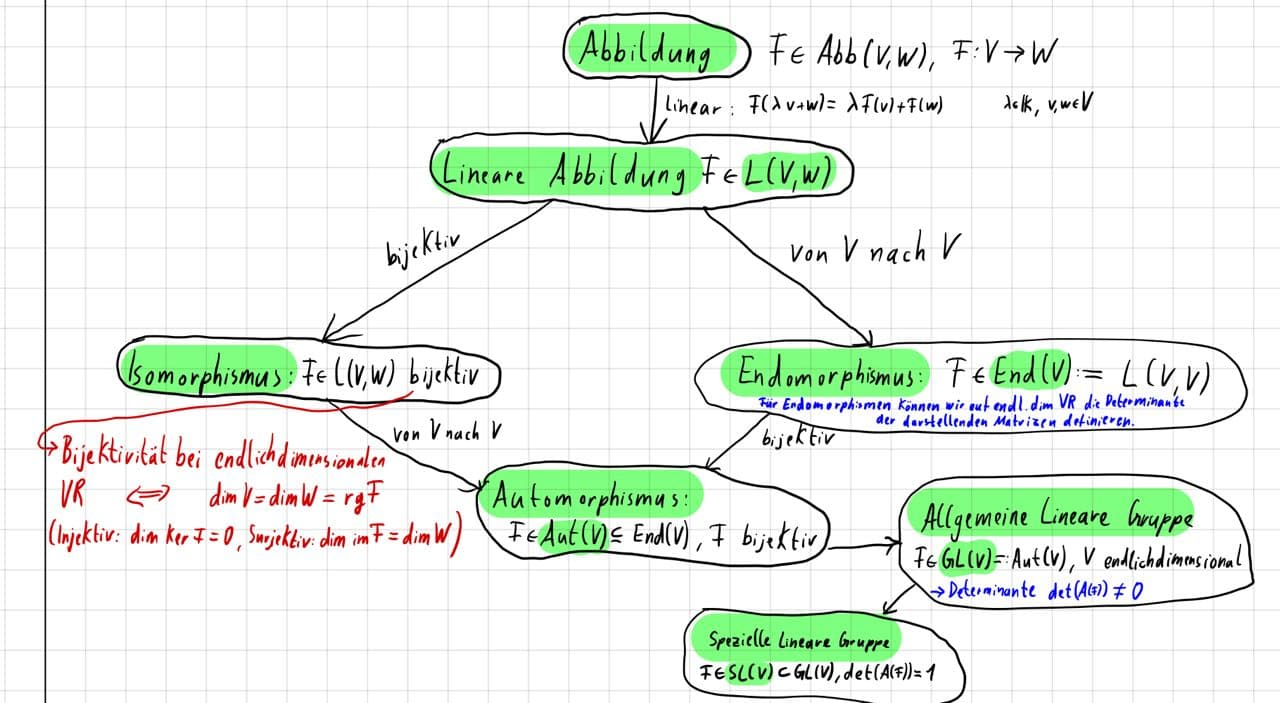
\includegraphics[width=.7\textwidth]{Dateien/01/01Wiederholung.jpg}
\end{center}

\begin{Wiederholung}
{Rang einer Matrix und einer Abbildung}
Der \red{Rang} einer Matrix entspricht der \underline{Anzahl an linear unabhängigen Spalten} (bzw. Zeilen) der Matrix.\\
Also ist der Rang die Anzahl der Zeilen, die nach Anwendung des Gauß-Algorithmus nicht 0 werden.\\
Wir ordnen jeder linearen Abbildung $F:V\to W$ die \underline{positive}\footnote{inklusive 0} ganze Zahl
\begin{equation}
    \boxed{\rg F=\dim(\im F)}
\end{equation}
zu und nennen diese den \red{Rang von $F$}.\\
Der Rang entspricht also der Dimension des Bildes. Er entspricht dem Rang einer beliebigen darstellenden Matrix von $F$.
\end{Wiederholung}
\begin{Wiederholung}{Dimensionsformel}
Für Vektorräume $V,W$ mit $\dim V=n\leq \infty$ und eine lineare Abbildung $F\in L(V,W)$ gilt:
\begin{equation*}
    \boxed{\rg F+\dim \ker F=\dim V}.
\end{equation*}
Die Dimension des Urbildraumes entspricht also der Summe aus der Dimension des Bildraumes und der Dimension des Raumes aller Vektoren aus $V$, die auf den Nullvektor abgebildet werden.
\end{Wiederholung}
Anschließend hatten wir die Determinante für Endomorphismen (bzw. deren darstellende Matrizen) eingeführt.
\begin{Wiederholung}{Wichtige Rechenregeln zu Determinanten}
Wie wir gesehen hatten, gilt für $A, B, \mathds{1}_n\in\mathbb{N}$:
\begin{itemize}
    \item $\det(\mathds{1}_n)=1$
    \item $\det(A)=\det(A^T)$
    \item $\det(AB)=\det(A)\det(B)$
    \item $\det(A^{-1})=\det(A)^{-1}$ falls $\det (A)\neq0$.
\end{itemize}
Zudem kennt ihr den Satz über Blockdreiecksmatrizen und wisst, dass ihr quasi die Gauß'schen Umformungen verwenden dürft.\footnote{Aber bei Multiplikation von Zeilen mit Skalaren immer schön drauf achten, die Determinante mit dem Inversen zu multiplizieren! Außerdem dürft ihr Zeilen/Spalten nur unter Hinzufügen eines Minuszeichens vertauschen.}\\
Zudem ist die Regel von Sarrus ein wichtiges Werkzeug für $3\times 3$-Matrizen, während die Determinante einer $2\times2$-Matrix ja einfach $ad-bc$ war.
\end{Wiederholung}

\subsection{Fortsetzung zu Determinanten - der Laplace'sche Entwicklungssatz}
Um den nächsten wichtigen Satz einzuführen, benötigen wir folgenden Begriff:
\begin{Def}
{Streichungsmatrix}
\begin{wrapfigure}{r}[0pt]{.35\textwidth}
 \vspace{-30pt}
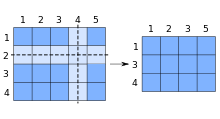
\includegraphics[width=.35\textwidth]{Dateien/01/01Submatrix_qtl1.svg.png}
 \vspace{-15pt}
\end{wrapfigure}
Für eine quadratische Matrix $A=(a_{kl})\in\Met(n,\mathbb{K})$ nennen wir $A_{ij}\in\Met(n-1,\mathbb{K})$ die ($i,j$)-te \red{Streichungsmatrix}\footnote{wobei $i,j\in\{1,...,n\}$. Dieser Begriff ist unter \href{https://de.wikipedia.org/wiki/Untermatrix}{Wikipedia} unter dem Namen 'Untermatrix' zu finden.}, die aus $A$ durch das Streichen der $i$-ten Zeile und $j$-ten Spalte entsteht.
\end{Def}
Durch den Laplace'schen Entwicklungssatz lässt sich die Berechnung der Determinante auf die Berechnung einiger 'kleinerer' Determinanten reduzieren.\\
Hierfür kann man eine Matrix $A$ nach der $i$-ten oder der $j$-ten Spalte \textit{entwickeln}:
\begin{Satz}{Satz}{Entwicklungssatz von Laplace}
Für die Determinante einer Matrix $A=(a_{kl})\in\Met(n,\mathbb{K})$ gilt
\begin{equation}
    \det A=\sum_{j=1}^n(-1)^{i+j}a_{ij}\det A_{ij}.
\end{equation}
\end{Satz}
Das sieht ziemlich wild aus, ist aber tatsächlich recht einfach:\\
Wir schnappen uns z.B. die erste Zeile und multiplizieren deren Einträge mit den Determinanten der Streichungsmatrizen und ggf. noch mit $(-1)$.
Wann ihr mit $(-1)$ multiplizieren müsst, könnt ihr euch nach folgendem Muster merken:
\begin{center}
    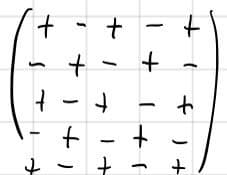
\includegraphics[width=.15\textwidth]{Dateien/01/01Laplacschema.jpg}
\end{center}
Es ist also immer alternierend.\\
\blue{\textbf{Hinweis}:\\
Es ist egal, nach welcher Zeile oder Spalte ihr entwickelt. Es lohnt sich häufig, gerade die Spalten/Zeilen zu wählen, die viele Nullen enthalten.}\\
Für das Beispiel, das wir auch im \textit{Determinanten}-Kapitel betrachtet hatten, sieht das dann so aus:
\begin{Beispiel}{Determinanten mit dem Entwicklungssatz berechnen}
Wir führen eine Entwicklung nach der ersten Zeile durch:
\begin{align*}
\det\Matrix{1&2&3\\4&5&0\\2&3&4}&=(-1)^{1+1}1\det\Matrix{5&0\\3&4}+(-1)^32\det\Matrix{4&0\\2&4}+3\det\Matrix{4&5\\2&3}\\
&=20-2\cdot16+3(12-10)=-12+6=-6.
\end{align*}
Alternativ können wir auch nach der dritten Spalte entwickeln:
\begin{align*}
\det\Matrix{1&2&3\\4&5&0\\2&3&4}&=(-1)^{1+3}3\det\Matrix{4&5\\2&3}+0+(-1)^{3+3}4\det\Matrix{1&2\\4&5}\\
&=3\cdot2+4(-3)=-6.
\end{align*}
\end{Beispiel}
Abschließend noch ein schönes Beispiel:
\begin{Beispiel}{Determinanten-Induktion}
\Zz{Für $n\in\mathbb{N}\setminus\{0\},\,a,b\in\mathbb{K}^n$ ist die Determinante einer Matrix $A$ der folgenden Gestalt durch
\begin{equation*}
    \det A=\det \Matrix{a_1&0&\cdots &\cdots&0&b_1\\
    0&\ddots&&&\iddots &0\\
    \vdots&&a_n&b_n&&\vdots\\
    \vdots&&b_n&a_n&&\vdots\\
    0&\iddots&&&\ddots &0\\
    b_1&0&\cdots &\cdots&0&a_1}=\prod_{k=1}^n(a_k^2-b_k^2)
\end{equation*}
gegeben.}
\Zb{Vollständige Induktion:\\
Induktionsanfang:\\
Für $n=1$ ist $\det A=\det\MatrixInline{a_1&b_1\\b_1&a_1}=a_1^2-b_1^2=\prod_{k=1}^n(a_k^2-b_k^2)$.\\
Es gelte die Induktionsvoraussetzung (siehe Aussage) für $n\geq 1$.\\
Induktionsschritt:\\
So folgt die Aussage für $n+1$, denn:
\begin{eqnarray*}
    \det A&=&\MatrixAbs{a_1&0&\cdots &\cdots&0&b_1\\
    0&\ddots&&&\iddots &0\\
    \vdots&&a_{n+1}&b_{n+1}&&\vdots\\
    \vdots&&b_{n+1}&a_{n+1}&&\vdots\\
    0&\iddots&&&\ddots &0\\
    b_1&0&\cdots &\cdots&0&a_1}\\
    &\overset{\footnote{Laplace-Entwicklung nach der $n+1$-ten Zeile}}{=}&a_{n+1}\MatrixAbs{a_1&0&\cdots &0&b_1\\
    0&\ddots&&\iddots &0\\
    \vdots&&a_{n+1}&&\vdots\\
    0&\iddots&&\ddots &0\\
    b_1&0&\cdots &0&a_1}-b_{n+1}\MatrixAbs{a_1&0&\cdots &0&b_1\\
    0&\ddots&&\iddots &0\\
    \vdots&&b_{n+1}&&\vdots\\
    0&\iddots&&\ddots &0\\
    b_1&0&\cdots &0&a_1}
\end{eqnarray*}
\begin{eqnarray*}
    &\overset{\footnote{Erneute Entwicklung nach der $n+1$-ten Zeile}}{=}&a_{n+1}^2\MatrixAbs{a_1&0&\cdots &\cdots&0&b_1\\
    0&\ddots&&&\iddots &0\\
    \vdots&&a_{n}&b_{n}&&\vdots\\
    \vdots&&b_{n}&a_{n}&&\vdots\\
    0&\iddots&&&\ddots &0\\
    b_1&0&\cdots &\cdots&0&a_1}-b_{n+1}^2\MatrixAbs{a_1&0&\cdots &\cdots&0&b_1\\
    0&\ddots&&&\iddots &0\\
    \vdots&&a_{n}&b_{n}&&\vdots\\
    \vdots&&b_{n}&a_{n}&&\vdots\\
    0&\iddots&&&\ddots &0\\
    b_1&0&\cdots &\cdots&0&a_1}\\
    &\overset{\footnote{Nutze die Induktionsvoraussetzung}}{=}&a_{n+1}^2\prod_{k=1}^n(a_k^2-b_k^2)-b_{n+1}^2\prod_{k=1}^n(a_k^2-b_k^2)\\
    &=&(a_{n+1}^2-b_{n+1}^2)\prod_{k=1}^n(a_k^2-b_k^2)\\
    &=&\prod_{k=1}^{n+1}(a_k^2-b_k^2)
\end{eqnarray*}}
\end{Beispiel}

\subsection{Zeit, umzukehren}
Wir betrachten nun einige Werkzeuge zum Invertieren von Matrizen. Dazu kurz nochmal ein Rückblick:
\begin{Wiederholung}{Lemma zur Bijektivität und Umkehrabbildung}\label{satz:BijektivitatUmkehrabbildung}
Eine Abbildung $f:A\rightarrow B$ ist \underline{genau dann bijektiv}, falls es eine Abbildung $g:B\to A$ gibt (diese nennen wir dann \red{Umkehrabbildung}), die die folgenden Relationen erfüllt:
\begin{equation}
    g\circ f=\text{Id}_A\,\wedge\, f\circ g=\text{Id}_B.\label{eq:Umkehrabbildung}
\end{equation}
\end{Wiederholung}
Wie wir schon festgestellt hatten, ist eine Matrix $A\in\Met(n,\mathbb{K})$ genau dann \red{invertierbar}, wenn $\det A\neq 0$.\\
Was bedeutet aber \textit{invertierbar}?
\begin{Wiederholung}{Inverse Matrix}
Ist $A$ invertierbar, so existiert eine \red{zu $A$ inverse Matrix $A^{-1}$}, sodass gilt:
\begin{equation}
    A\cdot A^{-1}=\mathds{1}_n\quad\tx{und}\quad A^{-1}\cdot A=\mathds{1}_n.
\end{equation}
\end{Wiederholung}
Falls $A$ die darstellende Matrix eines Endomorphismus ist, so ist dieser dann bijektiv und wir nennen ihn \red{Automorphismus}. Seht ihr die Parallelen zum Lemma zur Umkehrabbildung?\
\begin{Beispiel}{Inverse Matrix}
Sei $A=\Matrix{2&2\\3&4}$.\\
\Zz{Die Matrix $A^{-1}=\Matrix{2&-1\\-\frac{3}{2}&1}$ ist die zu $A$ inverse Matrix.}
\Zb{Es gilt 
\begin{equation*}
    A\cdot A^{-1}=\Matrix{2&2\\3&4}\Matrix{2&-1\\-\frac{3}{2}&1}=\Matrix{4-3&-2+2\\6-6&-3+4}=\Matrix{1&0\\0&1}=\mathds{1}_2
\end{equation*}
und analog andersherum.}
\end{Beispiel}

\begin{Wiederholung}{Inverse einer Determinante}
Für alle Gruppenhomomorphismen gilt $\phi(a^{-1})=\phi(a)^{-1}$. Somit gilt für alle\\
$A\in\GL(n,\mathbb{K})$:
\begin{equation}
    \det(A^{-1})=\det(A)^{-1}.
\end{equation}
Dies ist wohldefiniert, da $A\in\GL(n,\mathbb{K})$ per Definition bijektiv ist und somit eine Umkehrabbildung $A^{-1}$ besitzt und die Determinante nicht verschwindet.
\end{Wiederholung}
\begin{Wiederholung}
{Anwendung der Inversen Determinante}
Sei $A=\Matrix{2&2\\3&4}$. Die inverse Matrix ist (wie eben gesehen) $A^{-1}=\Matrix{2&-1\\-\frac{3}{2}&1}$.\\
Somit gilt:
\begin{align*}
    \det(A^{-1})&=2-(-1)(-3/2)=2-\frac{3}{2}=\frac{1}{2}\\
    \det(A)^{-1}&=(2\cdot 4-3\cdot 2)^{-1}=2^{-1}=\frac{1}{2}.
\end{align*}
\end{Wiederholung}
\begin{Def}
{Spezielle lineare Gruppe}
Wir bezeichnen die Untergruppe aller Automorphismen mit $\det A=1$ als \red{spezielle lineare Gruppe} und schreiben
\begin{equation}
    \SL=\Menge{A\in \GL(n,\mathbb{K})}{\det A=1}\subset \GL(n,\mathbb{K}).
\end{equation}
\end{Def}


\subsubsection{Invertieren mit dem Gauß-Verfahren}
Wie finden wir aber nun die inverse Matrix zu einer gegebenen Matrix $A$?
\begin{Satz}
{Rechenregel}{Invertieren einer Matrix mit Gauß}
Die erste Idee ist, dass wir ein Gleichungssystem umwandeln, indem wir mit $A^{-1}$ multiplizieren, d.h.
\begin{equation*}
    A\xvec=\Hat{\Vec{e}}_i\to \xvec=A^{-1}\Hat{\Vec{e}}_i.
\end{equation*}
Eine solche Überführung können wir durch den Gaußschen Algorithmus erreichen.\\
Um das für alle Spalten von $A^{-1}$ gleichzeitig zu machen, lösen wir also $(A\furdas\mathds{1}_n)\to(\mathds{1}_n\furdas A^{-1})$.
\end{Satz}
Das hört sich vielleicht komplizierter an, als es ist, daher hier ein Beispiel.
\begin{Beispiel}
{Invertieren einer Matrix mit Gauß}
Wir wollen die Matrix $A\in \GL(3,\mathbb{R}),\,A=\MatrixInline{1&2&3\\2&1&-1\\0&0&2}$ invertieren:
\begin{align*}
    (A\furdas\mathds{1}_3)&=\MatrixInvertieren{1&2&3\\2&1&-1\\0&0&2}{1&0&0\\0&1&0\\0&0&1}\overset{\tx{II}-2\tx{I},\, \tx{III }/2}{\longrightarrow}\MatrixInvertieren{1&2&3\\0&-3&-7\\0&0&1}{1&0&0\\-2&1&0\\0&0&1/2}\\
    \overset{\tx{I}-3\tx{III},\,\tx{II}+7\tx{III}}&{\longrightarrow}\MatrixInvertieren{1&2&0\\0&-3&0\\0&0&1}{1&0&-3/2\\-2&1&7/2\\0&0&1/2}\overset{\tx{II}/(-3)}{\longrightarrow}\MatrixInvertieren{1&2&0\\0&1&0\\0&0&1}{1&0&-3/2\\2/3&-1/3&-7/6\\0&0&1/2}\\
    \overset{\tx{I}-2\tx{II}}&{\longrightarrow}\MatrixInvertieren{1&0&0\\0&1&0\\0&0&1}{-1/3&2/3&5/6\\2/3&-1/3&-7/6\\0&0&1/2}=(\mathds{1}_3\furdas A^{-1}).
\end{align*}
Somit ist $A^{-1}=\frac{1}{6}\MatrixInline{-2&4&5\\4&-2&-7\\0&0&3}$ die zu $A$ inverse Matrix.\\
Wie können wir das testen?
\begin{itemize}
    \item \textbf{Überprüfe die Determinanten}:\\
    $\det(A^{-1})\overset{!}{=}(\det A)^{-1}$. Es ist
    \begin{eqnarray*}
        \det(A^{-1})&\overset{\footnote{Regel von Sarrus, Linearität}}{=}&\BracedIn{\frac{1}{6}}^3\BracedIn{(-2)(-2)3-4\cdot4\cdot3}=\frac{1}{36}\BracedIn{2-8}=-\frac{6}{36}=-\frac{1}{6}.\\
        \det A&=&1\cdot 1\cdot 2-2\cdot 2\cdot 2=2-8=-6\implies (\det A)^{-1}=-\frac{1}{6}.
    \end{eqnarray*}
    Leider ist dieses Kriterium nur notwendig, aber nicht hinreichend. Es kann aber als schneller Test dienen.
    \item \textbf{Stumpf rechnen}:\\
    Wir berechnen einfach
    \begin{equation*}
        A\cdot A^{-1}=\frac{1}{6}\Matrix{-2&4&5\\4&-2&-7\\0&0&3}\Matrix{1&2&3\\2&1&-1\\0&0&2}\overset{\footnote{Wir tun an dieser Stelle einfach mal so, als hätten wir das wirklich gerechnet ;)}}{=}\Matrix{1&0&0\\0&1&0\\0&0&1}.
    \end{equation*}
    Dieses Kriterium ist dann sowohl notwendig als auch hinreichend.
\end{itemize}
\end{Beispiel}

\subsubsection{Invertieren mit der Adjunkten}
Es gibt eine weitere, unintuitivere Möglichkeit, Matrizen zu invertieren. Hierfür benötigen wir den Begriff der adjunkten Matrix:
\begin{Def}
{Adjunkte Matrix}
Für die Matrix $A=(a_{ij})_{ij}\in\Met(n,\mathbb{K})$ definieren wir die \red{adjunkte Matrix} $\Tilde{A}=(\Tilde{a}_{ij})_{ij}$, die die folgenden Einträge hat:
\begin{equation*}
    \Tilde{a}_{ij}=(-1)^{i+j}\det A_{ji}=\det(\Vec{a}_1\ldots\Vec{a}_{i-1}\Vec{e}_j\Vec{a}_{i+1}\ldots a_n),
\end{equation*}
wobei $A_{ji}$ die $ji$-te Streichungsmatrix ist.
\end{Def}
Das sieht auf den ersten Blick erst mal ungewohnt aus, also betrachten wir es genauer:
\begin{Beispiel}
{Adjunkte einer $2\times 2$-Matrix (1/2)}
Sei $A=\MatrixInline{a&b\\c&d}$, so finden wir
\begin{equation*}
    \Tilde{a}_{11}=(-1)^2\det d,\quad \Tilde{a}_{12}=(-1)^3\det b,\quad \Tilde{a}_{21}=(-1)^3\det c,\quad \Tilde{a}_{22}=(-1)^4\det a. 
\end{equation*}
Somit ist $\Tilde{A}=\MatrixInline{d&-b\\-c&a}$.
\end{Beispiel}
\begin{Beispiel}
{Adjunkte einer $3\times 3$-Matrix (2/2)}
Sei $A=\MatrixInline{a&b&c\\d&e&f\\g&h&i}$, so finden wir
\begin{equation*}
    \Tilde{a}_{11}=(-1)^2\det \Matrix{e&f\\h&i},\quad \Tilde{a}_{12}\overset{\footnote{Streichungsmatrix 2. Zeile, 1. Spalte}}{=}(-1)^3\det \Matrix{b&c\\h&i},\quad \Tilde{a}_{13}=(-1)^4\det\Matrix{b&c\\e&f}
\end{equation*}
und so weiter...
\end{Beispiel}
\begin{Satz}
{Satz}{Zur adjunkten Matrix}
Für die adjunkte Matrix $\Tilde{A}$ zu $A\in \Met(n,\mathbb{K})$ gilt:
\begin{equation}
    A\cdot \Tilde{A}=\det A\mathds{1}_n\quad\tx{und}\quad \Tilde{A}\cdot A=\det A\mathds{1}_n.
\end{equation}
\end{Satz}
Wir sehen also, dass die Adjunkte quasi die Struktur der inversen Matrix hat, jedoch um einen Faktor $\det A$ daneben liegt.
\begin{Satz}
{Rechenregel}{Cramersche Regel zur Bestimmung der inversen Matrix}
Mithilfe der Adjunkten können wir aufgrund des vorhergehen Satzes also leicht die inverse Matrix einer invertierbaren Matrix $A\in\GL(n,\mathbb{K})$ bestimmen, denn es gilt
\begin{equation}
    \boxed{A^{-1}=\frac{1}{\det A}\Tilde{A}}.
\end{equation}
\end{Satz}
Der folgende Satz ist recht wichtig, es lohnt sich, ihn auswendig zu lernen:
\begin{Satz}
{Merksatz}{Inverse einer $2\times2$-Matrix}
Sehr häufig braucht man das Inverse einer $2\times2$-Matrix $A=\MatrixInline{a&b\\c&d}$.\\
Mithilfe der Adjunkten sehen wir:
\begin{equation}
    \label{eq:01InverseZweiKreuzZwei}A^{-1}=\frac{1}{\det A}\Tilde{A}=\frac{1}{ad-bc}\Matrix{d&-b\\-c&a}.
\end{equation}
\end{Satz}

\Tipps{1}{
\begin{enumerate}
    \item Die Formulierung ist vielleicht etwas ungewohnt, aber fasst einfach die Polynome als Vektor auf und sucht euch zunächst ein Beispiel.\\
    Auf was wird z.B. das Polynom $P(x)=5+7x-3x^3=\MatrixInline{5\\7\\0\\-3}$ durch die Ableitung abgebildet?\\
    Dann müsst ihr euch überlegen, wie ihr diese lineare Abbildung mithilfe einer Matrix aufschreiben könnt.\\
    Alternativ könnt ihr auch ganz klassisch schauen, was die Ableitung mit den Basisvektoren der Basis $(1,x,x^2,x^3)$ macht, und wie ihr das Ergebnis durch diese wieder darstellen könnt. Spaltenweise aufgeschrieben ergibt das dann eure Matrix.\\
    Spur und Determinante sollten ein Kinderspiel sein.
    \item Erinnert euch an die Unterraumaxiome. Diese müsst ihr überprüfen. Das sieht auf den ersten Blick vielleicht kompliziert aus, gestaltet sich aber letztlich als (einigermaßen) kurze Rechnung.
    \item Auch bei dieser Aufgabe handelt es sich um relativ kurze Rechnungen. Bei a.) erinnert euch einfach daran, wie Linearität definiert ist. Auch bei b.) schaut euch an, was für Matrizen gelten muss, die im Kern von $\varphi$ liegen und welche Bedingungen daraus für die Matrixelemente folgen. In c.) müsst ihr das Bild auf Symmetrie untersuchen und euch überlegen, wie man beliebige symmetrische Matrizen so zerlegen kann, dass sie ein Bild von $\varphi$ sind. Für d.) schaut euch nochmal die Körperaxiome an. 
    \item Der erste Teil ist schnell gemacht.\\
    Welche Bedingungen für $a, b,c$ und $d$ folgen aus den Forderungen? Ihr solltet nur noch zwei freie Variablen haben.\\
    Der letzte Teil sollte damit dann auch schnell gehen.
    \item Dies ist ein Einzeiler. Startet mit der Definition des Betrages und macht euch dann klar, wie eine Matrix mit $(\overline{u_{ji}})$ aussieht.
\end{enumerate}
}